

\subsection{Existing Approaches}

We investigate existing approaches that target on reducing the sensitivity and classify them into offline ones and online ones, where the former chases to reduce the sensitivity by exploring better model parameters and the latter pursues insensitivity by unification or simplification of input data. Thus, data processing steps are required before inputting into the model and after the inference during the test time and speaker names in $D_{tr}$, $D_{va}$ and $D_{te}$ are all changed for online approaches.
The model needs fine-tuning for both approaches. 

%Offline approaches fine-tune models to be more insensitive to speaker names. 
%No extra steps are required when using the model during the test time.

\textit{Offline approaches} include:


\textbf{Embedding Layer(Emb)}: Similar to~\cite{gu2020speaker} and ~\cite{heetal2021speakerturn}, an additional embedding layer can be adopted for representing whether the model should be sensitive to corresponding tokens. $2$ embeddings are learned during fine-tuning. 

\textbf{Augmentation (Aug)}: \citet{liu2021controllable} proposed to do data augmentation by exchanging speaker names in training samples with names from $D_{tr}$. They aim to reduce unexpected inductive bias caused by speaker names, which is similar to our goal. The model is fine-tuned with augmented training data while $D_{va}$ and $D_{te}$ remain unchanged.

%\textbf{Insensitivity Loss (Ins)}: We newly propose a fine-tuning objective on top of the augmented data in Fig.~\ref{fig:insloss}. More details are in Sec.~\ref{sec:insloss}.% shown in Figure~\ref{fig:insloss}, helping to reduce sensitivity with augmented data (More in ~\ref{sec:insloss}).


%\subsection{Online Approaches}
%\label{sec:dda}
\textit{Online approaches} are:
%also need fine-tuning. The main difference is that data processing steps are required before inputting into the model and after the inference during the test time. Speaker names in $D_{tr}$, $D_{va}$ and $D_{te}$ are all changed.%Two approaches are as follows.

\textbf{ID:} Some works~\cite{cui2020mutual,li2017dailydialog} replace speaker names with predefined IDs to avoid name bias.
We use ``Speaker[NUM]'' similarly to \citet{kim2019eighth} and \citet{chen2021dialogsum}, 
which is close to words seen during pre-training and fits different numbers of speakers.
``[NUM]'' is the index of a speaker's first occurrence. 

\textbf{Frequent (Fre)}: This refers to the approach proposed in \citet{khalifa2021bag}. They use 100 frequent male and 100 frequent female names online\footnote{https://www.ssa.gov/oact/babynames/decades/century.html} as the pool $P$ for sampling replacements. This approach can be combined with Aug into \textbf{FreAug}.




\section{Proposed Approach}
\label{sec:approach}


%\begin{figure*}[th]
%	\centering
%	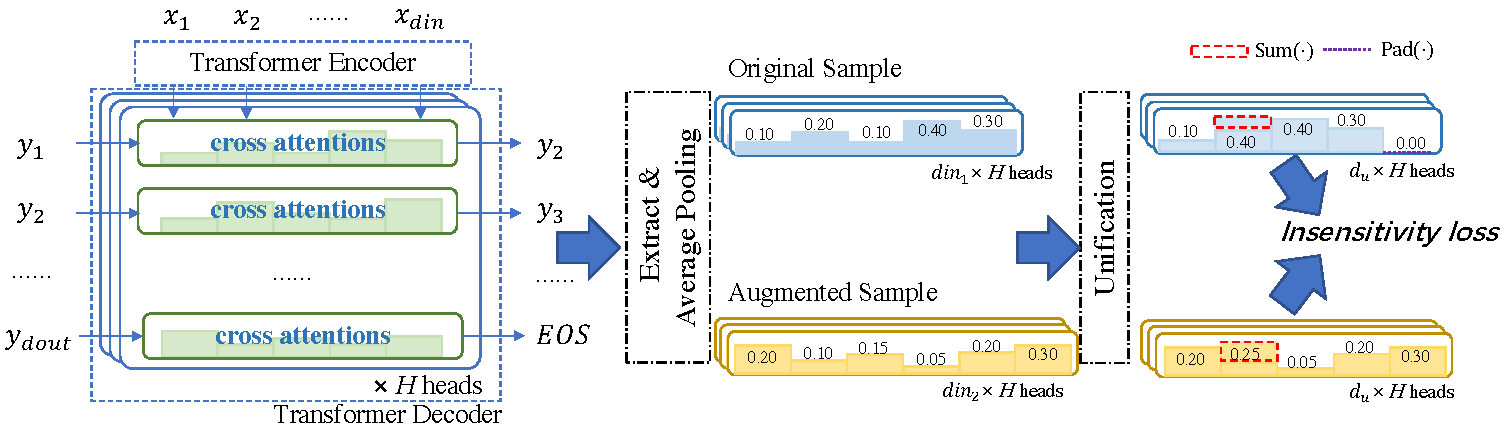
\includegraphics[scale=0.6]{insloss.pdf}
%	\caption{An illustration of our Insensitivity Loss when $K=2$.
%	}
%	\label{fig:insloss}
%\end{figure*}


%Previous approach Aug only tries to reduce undesired biases with more data while neglects the model itself. 
We focus on the widely-accepted encoder-decoder architecture for pre-trained generation models and design two auxiliary insensitivity losses to take full advantage of augmented data on top of Aug. 
Given the dialogue sample with different speaker names, a model outputs distinct generations due to its different internal behaviors. Therefore, penalizing unexpected internal differences should help the model behave consistently and reduce the sensitivity.
 
With this intuition, we propose the cross-attention loss and the decoder-hidden-state loss. 
The former corresponds to cross-attention distributions that help the decoder make a soft information selection among encoder hidden states at each step and should be similar with different speaker names. 
%Thus, narrowing down the differences of such hidden information selection reflected by attention distributions is necessary. 
The latter is based on the final decoder hidden states which are expected to be the same under the default teacher-forcing training strategy except for the speaker name tokens.
We didn't consider the encoder attentions since according to our pilot analysis of the vanilla BART, %with pairs of samples, 
the cross attentions distance of the different predictions is around 1.5 times of the same ones. However, there are no differences in the encoder attentions. 
Other intermediate hidden states are excluded since they are all affected by different input embeddings of speaker names, except that the final decoder hidden states are sure to be the same.% to get identical predictions. %More details are as follows. %detailed explanations for two losses are as follows.

%The main intuition is to penalize the unexpected differences of model's internal behavior among the same dialogue samples with different speaker names.



%On top of the previous approach Aug, we propose two new auxiliary losses to train more insensitive models: the cross-attention insensitivity loss and the decoder-hidden-state insensitivity loss. The intuition for both losses are to penalize the differences of model's internal behavior among the same dialogue samples with different speaker names.
%More details are as follows.
%Then, we propose two insensitivity losses to further reduce the sensitivity. 

%The encoder-decoder architecture is the most widely-accepted design for pre-trained generation models. 
%At each time step, the decoder selects information to concentrate on among the encoder hidden states with the cross-attention mechanism, and predicts the current output. This soft information selection process determines the contents included in the final predictions. 
%The intuition here is to narrow down the differences of such hidden information selection reflected by attention distributions.

\subsection{Cross-attention Insensitivity Loss}
\label{sec:insloss}


%\JQ{design space: input, cross attention, decoder}
%We did a pilot experiment on the SAMSum dataset with vanilla fine-tuned BART. By switching names, we collect two generations for each sample. Among the 71.92\% samples with different outputs, we randomly sampled 200 pairs and asked human annotators to label each case among 4 types (More details are in the Appendix). The Kappa score is 95.94\% with perfect agreement. 

%According to the pilot experiment metioned in Sec.~\ref{sec:intro}(More details are in the Appendix), the results shows that the most severe sensitivity is from content distinction, meaning that generations contain different information or keywords. This inspired us to design the following loss function.





%We denote the input and output of a transformer-based model as $X=\{x_1, x_2, ..., x_{din} \}$ and $Y=\{y_1, y_2, ..., y_{dout}\}$ respectively. $din$ and $dout$ represent the number of corresponding tokens.
We denote a model's input and output length, i.e., the number of tokens, as $din$ and $dout$.
During training, the cross attentions calculated for each output token are collected as $CA\in R^{N\times dout \times din}$. $N$ is the number of heads for the multi-head attention mechanism, determined by the configuration of pre-trained models. We apply average pooling over the dimension of $dout$, to get the overall attention over the input tokens $\overline{CA}\in R^{N\times din}$.
% $\rm{avg}(\cdot)$

Given an original sample $\{d_i, c_i, o_i\}$, we construct $K-1$ augmented samples by replacing speaker names. The averaged attentions for all samples are $\{\overline{CA_k}\}_{k=1}^K$. Since it is a default that each sample should go through the tokenizer before inputting to the model, $\{din_k\}_{k=1}^K$ are not guaranteed to be identical in two cases.
%. The lengths of the two distributions are different in two cases. 
First, names may be tokenized into different token counts. For example, ``John'' and ``Robinson'' are tokenized into \{``John''\} and \{``Rob'', ``inson''\} by BART tokenizer. Replacing ``John'' with ``Robinson'' in $d_i$ will increase the sequence length. Second, long inputs may be truncated at different tokens. So, we consider two corresponding functions for unification: %before calculating the distance of these distributions. %We consider two corresponding functions:
\begin{itemize}
\item $\rm{Sum(\cdot)}$ sums up the attention values of tokens belonging to an occurrence of a speaker name. 
\item $\rm{Pad(\cdot)}$ pads attentions into the same length $din_u$ by concatenating zeros, which means that this part of contents is missing.% due to truncation.
%\begin{itemize}
%	\item 
%	\item 
\end{itemize}
The unified $\{\overline{CA_k}\}_{k=1}^K$ is represented as $\{\widetilde{CA}_k\}_{k=1}^K$, where $\widetilde{CA}_k\in R^{N\times din_u}$.


Finally, the loss is calculated as:
\begin{equation}
	\mathcal{L}_{ca} = \frac{1}{K(K-1)} \sum_{k=1}^{K}\sum_{l=1, l\neq k}^{K} {loss}(\widetilde{CA}_k, \widetilde{CA}_l)
\end{equation}
where ${loss}(\cdot)$ measures the distances between a pair of attentions. 

\subsection{Decoder-hidden-state Insensitivity Loss}

Similarly, hidden states of the decoder's final output for all samples can be denoted as $\{DH_k\}_{k=1}^K$, where $DH_k\in R^{H\times dout_k}$ and $H$ represents the hidden size. The lengths of them also vary due to the above two cases. We adopt two different functions: %for unification:
\begin{itemize}
	\item $\rm{Del(\cdot)}$ ignores the hidden states whose predicted tokens belong to a speaker name.
	\item $\rm{Trunc(\cdot)}$ truncates the redundant hidden states at the end without the paired ones.
\end{itemize}
Thus, the unified $\{DH_k\}_{k=1}^K$ is represented as $\{\widetilde{DH}_k\}_{k=1}^K$, where $\widetilde{DH}_k\in R^{H\times dout_u}$.

The loss is defined as:
\begin{equation}
	\mathcal{L}_{dh} = \frac{1}{K(K-1)} \sum_{k=1}^{K}\sum_{l=1, l\neq k}^{K} loss(\widetilde{DH}_k, \widetilde{DH}_l)
\end{equation}
We adopted the mean square error for both losses.

\subsection{Learning Objective}


$\mathcal{L}_{ca}$ and $\mathcal{L}_{dh}$ are added to the vanilla generation loss $\mathcal{L}_{gen}$ with hyper-parameters $\alpha$ and $\beta$: %newly-introduced
\begin{equation}
	\begin{aligned}
		%\mathcal{L}_{gen} =  \frac{1}{K}\sum_{k=1}^{K} \rm{loss}_{gen}(d_i^k, o_i^k) \\
		\mathcal{L}_{total} = \mathcal{L}_{gen} + \alpha \mathcal{L}_{ca} + \beta \mathcal{L}_{dh}
	\end{aligned}
\end{equation}
The insensitivity losses are only auxiliary fine-tuning objectives, leaving the inference time unchanged. They can be added on top of both Aug and FreAug, denoted as \textbf{Ins} and \textbf{FreIns}.

%We also compared the attention distance in this way of output pairs mentioned above. It shows that the attention distance for pairs with different outputs is 1.3~2.3 times of the same ones.

